\documentclass[master=cws,masteroption=ai,ascii,utf8]{kulemt}
\setup{title={Automatisch vertalen van logigrammen naar logica},
  author={Jens Claes},
  promotor={Prof. dr. M. Denecker},
  assessor={Ir.\,W. Eetveel\and W. Eetrest},
  assistant={Ir. L. Janssens}}
% De volgende \setup mag verwijderd worden als geen fiche gewenst is.
\setup{filingcard,
  translatedtitle={Automatic translation of logigrams into logic},
  udc=621.3,
  shortabstract={Hier komt een heel bondig abstract van hooguit 500
    woorden. \LaTeX\ commando's mogen hier gebruikt worden. Blanco lijnen
    (of het commando \texttt{\string\pa r}) zijn wel niet toegelaten!
    \endgraf \lipsum[2]}}
% Verwijder de "%" op de volgende lijn als je de kaft wil afdrukken
%\setup{coverpageonly}
% Verwijder de "%" op de volgende lijn als je enkel de eerste pagina's wil
% afdrukken en de rest bv. via Word aanmaken.
%\setup{frontpagesonly}

% Kies de fonts voor de gewone tekst, bv. Latin Modern
\setup{font=lm}

% Hier kun je dan nog andere pakketten laden of eigen definities voorzien
\usepackage[dutch]{babel}
\usepackage{pgf-pie}
\usepackage{url}
\usepackage[T1]{fontenc}
% \usepackage[utf8]{inputenc}
\usepackage{amsthm}
\usepackage{amsmath}
\usepackage{qtree}
\usepackage{footnote}

\theoremstyle{definition}
\newtheorem{ex}{Voorbeeld}[section]

\newcommand{\example}[1]{\textit{``#1''}}
\newcommand{\fstructure}[1]{\left [\begin{tabular}{lr}#1\end{tabular}\right]}
\newcommand{\feature}[2]{#1 & #2 \\}
\newcommand{\fvariable}[1]{\framebox{#1}}


% Tenslotte wordt hyperref gebruikt voor pdf bestanden.
% Dit mag verwijderd worden voor de af te drukken versie.
\usepackage[pdfusetitle,colorlinks,plainpages=false]{hyperref}

%%%%%%%
% Om wat tekst te genereren wordt hier het lipsum pakket gebruikt.
% Bij een echte masterproef heb je dit natuurlijk nooit nodig!
\IfFileExists{lipsum.sty}%
 {\usepackage{lipsum}\setlipsumdefault{11-13}}%
 {\newcommand{\lipsum}[1][11-13]{\par Hier komt wat tekst: lipsum ##1.\par}}
%%%%%%%

%\includeonly{hfdst-n}
\begin{document}

\begin{preface}
  Dit is mijn dankwoord om iedereen te danken die mij bezig gehouden heeft.
  Hierbij dank ik mijn promotor, mijn begeleider en de voltallige jury.
  Ook mijn familie heeft mij erg gesteund natuurlijk.
\end{preface}

\tableofcontents*

\begin{abstract}
  In dit \texttt{abstract} environment wordt een al dan niet uitgebreide
  samenvatting van het werk gegeven. De bedoeling is wel dat dit tot
  1~bladzijde beperkt blijft.

  \lipsum[1]
\end{abstract}

% Een lijst van figuren en tabellen is optioneel
%\listoffigures
%\listoftables
% Bij een beperkt aantal figuren en tabellen gebruik je liever het volgende:
\listoffiguresandtables
% De lijst van symbolen is eveneens optioneel.
% Deze lijst moet wel manueel aangemaakt worden, bv. als volgt:
\chapter{Lijst van afkortingen en symbolen}
\section*{Afkortingen}
\begin{flushleft}
  \renewcommand{\arraystretch}{1.1}
  \begin{tabularx}{\textwidth}{@{}p{12mm}X@{}}
    CNL   & Constructed Natural Language \\
    KBS   & Knowledge base paradigma \\
  \end{tabularx}
\end{flushleft}
\section*{Constituenten}
De verschillende soorten constituenten die kunnen voorkomen in een grammatica (terminologie uit de taalkunde). We gebruiken de Engelse namen voor gelijkaardigheid met de literatuur.
\begin{flushleft}
  \renewcommand{\arraystretch}{1.1}
  \begin{tabularx}{\textwidth}{@{}p{12mm}X@{}}
    s     & Sentence (zin) \\
    np    & Noun Phrase (naamwoordgroep) \\
    vp    & Verb Phrase (verbale constituent) \\
    v     & Verb (werkwoord) \\
    n     & Noun (zelfstandig naamwoord) \\
    det   & Determinator \\
  \end{tabularx}
\end{flushleft}

% \section*{Symbolen}
% \begin{flushleft}
%   \renewcommand{\arraystretch}{1.1}
%   \begin{tabularx}{\textwidth}{@{}p{12mm}X@{}}
%     $m$   & Massa \\
%   \end{tabularx}
% \end{flushleft}


\chapter{Inleiding}
\paragraph{} Logigrammen zijn een soort van puzzels waarbij de lezer een aantal zinnen voorgeschoteld krijgt. De zinnen bevatten een aantal domeinen (zoals nationaliteit, dier, kleur, ...) en een aantal domeinelementen (Noor, Brit, kat, hond, rood, blauw, ...). Ze beschrijven één bijectie tussen elk paar van domeinen. Het doel van de puzzel is het achterhalen van de waarde van de bijecties. M.a.w. welke domeinelementen bij elkaar horen. Bijvoorbeeld ``De Noor woont in het blauwe huis en heeft een kat als huisdier''. Elke puzzel heeft exact één oplossing.

De zinnen van logigrammen zijn redelijk gestructureerd waardoor het mogelijk is om ze automatisch om te vormen naar een formele representatie waarop inferenties uitgevoerd kunnen worden. Deze thesis onderzoekt hoe haalbaar deze automatische vertaling van logigrammen naar logica is. Dit dient als opstap naar meer algemene vertalingen van een natuurlijke taal naar een formele taal.

\paragraph{} We bestuderen hiervoor het framework van Blackburn en Bos \cite{Blackburn2005, Blackburn2006}. Dit framework is gebaseerd op lambda-calculus en Frege's compositionaliteitsprincipe (de betekenis van een woordgroep is een combinatie van de betekenissen van de woorden of woordgroepen waaruit ze bestaat).

We geven eerst wat achtergrond die kan helpen bij het begrijpen van de thesis. Dan beschrijven we een aantal vertalingen van een natuurlijke taal naar een formele taal uit de literatuur. Daarna overlopen we het systeem dat we gebruiken om logigrammen automatisch op te lossen. Vervolgens stellen we het framework van Blackburn en Bos voor en leggen we uit hoe we dit framework kunnen gebruiken voor het vertalen van logigrammen naar logica. Eerst bespreken we het lexicon, vervolgens de grammatica. Daarna breiden we het framework uit met types en vervolgens illustreren we hoe we a.d.h.v. deze types een volledige specificatie kunnen opstellen. Ter evaluatie passen we dit hele framework toe op een aantal logigrammen uit Puzzle Baron's Logic Puzzles Volume 3 \cite{logigrammen}.

\chapter{Motivatie}

\paragraph{} Vele bedrijfsprocessen worden geregeld door specificaties. Deze worden vaak geschreven in een natuurlijke taal, door een domein expert. Vervolgens worden deze specificaties vertaald naar uitvoerbare programma's. Bij deze vertaling kunnen er fouten insluipen. Bovendien zijn er vaak meerdere programma's die elk opnieuw de specificatie moeten implementeren. Zo ontstaan er niet alleen inconsistenties met de specificatie, maar ook tussen de verschillende programma's onderling. Ten slotte is het moeilijk om de specificatie achteraf nog aan te passen omdat alle programma's dan aangepast moeten worden.

\paragraph{} Het antwoord van de academische wereld op deze problemen, is het \textit{Knowledge Base}-paradigma. In dit paradigma staat een kennisbank centraal. Deze kennisbank bevat de kennis over de wereld en vormt een specificatie van hoe een systeem zich zou moeten gedragen. Deze kennisbank kan dan gebruikt worden in een \textit{Knowledge Base System (KBS)}. Zo'n systeem biedt een aantal inferenties aan die toegepast kunnen worden op deze kennisbanken. De Cat et al. \cite{IDP} geven het voorbeeld van een KBS dat gebruikt wordt om de vakken van een universiteit te beheren. De kennisbank in zo'n systeem bevat regels als ``In elk lokaal en op elk moment mag er maximum één les plaatsvinden''. Het systeem kan dan verschillende inferenties hierop uitvoeren. De Cat et al. geven de voorbeelden van \textit{propagatie} (bijvoorbeeld in het individuele studieprogramma van een student automatisch de vakken toevoegen die een vereiste zijn om andere vakken te volgen die expliciet door de student werden gekozen), \textit{model expansie} (bijvoorbeeld het opstellen van een volledig studieprogramma op basis van een partieel programma) en \textit{bevraging} (bijvoorbeeld het opvragen van een uurrooster voor een specifieke student).

Op basis van de output van de inferenties kunnen de bedrijfsprocessen dan geregeld worden. Om de kennis voor te stellen, kan men gebruik maken van een formele taal (zoals eerste-orde-logica). Zo'n talen hebben een eenduidige semantiek. Er is dus maar \'e\'en mogelijke manier waarop een zin ge\"interpreteerd kan worden. Dit in tegenstelling tot natuurlijke talen waar zelfs simpele zinnen al snel ambigu zijn.

In het Knowledge Base-paradigma moet de specificatie in natuurlijke taal (geschreven door een domein expert) vertaald worden naar een vorm waar het KBS mee overweg kan: de formele specificatie. Deze specificatie wordt slechts eenmaal geschreven en vervolgens wordt ze gebruikt voor alle soorten inferenties. Daardoor is het niet meer mogelijk dat de programma's onderling inconsistent zijn. Ze gebruiken namelijk allemaal dezelfde formele specificatie. Bovendien is ook het aanpassen van de specificatie makkelijker. Enkel de specificatie moet aangepast worden, de programma's blijven hetzelfde.

\paragraph{} Het probleem met deze aanpak is dat er nog steeds een vertaling moet gebeuren van natuurlijke taal naar een formele taal. De specificatie in natuurlijke taal wordt vaak opgesteld door een domein expert die niet vertrouwd is met formele talen. De formele specificatie wordt dan weer opgesteld door een KBS expert. Deze persoon kent formele talen maar heeft een beperkte kennis van het domein. Door deze mismatch van expertise, sluipen er fouten in de vertaling. De domein expert kan namelijk de subtiliteiten van de formele taal niet lezen. Vice versa kent de KBS expert de subtiliteiten van het domein niet.

\paragraph{} De vraag rijst dus of we een formele taal kunnen ontwerpen die toegankelijk is voor domein experten, rijk genoeg is voor praktische problemen en toepasbaar is binnen het KBS paradigma.

Deze thesis onderzoekt of een formele natuurlijke taal het antwoord is op die vraag. Hieronder verstaan we (een subset van) een natuurlijke taal met een formele, eenduidige semantiek. Talen die een subset zijn van een natuurlijke taal worden ook wel gecontroleerde natuurlijke talen of CNL's (naar het Engelse \textit{Controlled Natural Language}) genoemd. Deze talen verschillen van hun gasttaal doordat ze een aantal zinsconstructies niet toelaten. Dit kan bijvoorbeeld de leesbaarheid van een taal verhogen. Voor dit onderzoek zijn deze talen interessant omdat ambigue constructies op die manier verboden kunnen worden. Bovendien is de grammatica van een CNL veel simpeler dan die van de volledige natuurlijke taal, waardoor het makkelijker is om er een parser voor te schrijven. De zinnen die toegestaan zijn in de CNL worden vaak beschreven in een set van \textit{constructieregels}.

Naast constructieregels bevat een formele natuurlijke taal vaak ook interpretatieregels. Deze laatste bepalen hoe een zin die ambigu is in de gasttaal, ge\"interpreteerd moet worden in de nieuwe taal. De moeilijkheid ligt erin om deze regels te beperken in aantal en in complexiteit, zodanig dat de geconstrueerde taal zo dicht mogelijk tegen de gasttaal aanleunt.

% \paragraph{} We zullen deze formele natuurlijke taal opstellen binnen het domein van logigrammen. Hierbij zullen de constructieregels en interpretatieregels zodanig moeten opgesteld worden dat ze de betekenis van de logigrammen juist omzetten naar een formele representatie.

Het grote voordeel van een formele natuurlijke taal is dat natuurlijke taal al gebruikt wordt bij het opstellen van de specificatie. Een voorbeeld van een domein waar specificaties een grote rol spelen is vereistenanalyse. Hier zien we dat specificaties vaak in natuurlijke taal worden opgesteld. Zo toont figuur \ref{fig:natural-language-use} het gebruik van natuurlijke taal in vereistenanalyse in 1999 \cite{Luisa2004}. Slechts 5 procent van de specificaties werd toen in een formele taal opgesteld. Al de rest werd in een natuurlijke taal geformuleerd. 16 procent werd zelfs al in een gecontroleerde natuurlijke taal opgesteld.

\begin{figure}
  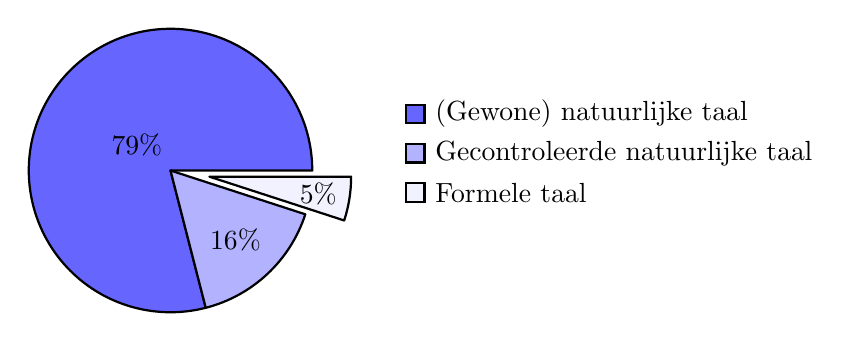
\begin{tikzpicture}
      \pie[text = legend, radius = 1.8, explode = {0, 0, 0.5}, color = {blue!60, blue!30, blue!5}]{79/(Gewone) natuurlijke taal, 16/Gecontroleerde natuurlijke taal, 5/Formele taal}
  \end{tikzpicture}
  \caption[Gebruik van natuurlijke taal in vereistenanalyse]{Gebruik van natuurlijke taal in vereistenanalyse in 1999 (van figuur 5 in \cite{Luisa2004})}
  \label{fig:natural-language-use}
\end{figure}

\paragraph{} We voeren ons onderzoek naar zo'n formele natuurlijke taal uit binnen het domein van logigrammen. Ze kunnen namelijk aanzien worden als kleine specificaties. Bovendien kunnen ze uitgedrukt worden in relatief simpele logische zinnen. Ten slotte kan men makkelijk vele voorbeelden vinden van zo'n logigrammen. We zullen hierbij zelf geen grammatica opstellen maar een aantal grammaticale regels afleiden van bestaande logigrammen (uit Puzzle Baron's Logic Puzzles Volume 3 \cite{logigrammen}).

\chapter{Achtergrond}
Om deze thesis te begrijpen worden hier een aantal concepten uitgelegd die niet per se tot de achtergrondkennis behoren van de lezer. Definite Clause Grammars zijn een soort van grammatica die een aantal voordelen biedt voor het parsen van natuurlijke taal. Feature structures zorgen voor een beperking van het aantal grammaticale regels en verhogen de leesbaarheid ervan. Discourse Representation Theory is een theorie uit de taalkunde voor het vatten van de betekenis van taal. Het introduceert Discourse Representation Structures, een logica die dichter aanleunt bij de natuurlijke taal.

\section{Definite Clause Grammars}
\label{sec:DCG}
Definite Clause Grammars \cite{Pereira1980} zijn een uitbreiding van contextvrije grammatica's die vaak ingebakken zitten in logische talen zoals prolog. Pereira et al.\ \cite{Pereira1980} geven 3 voorbeelden van hoe DCG's kunnen helpen bij het parsen van natuurlijke talen:

\begin{enumerate}
  \item De woordvorm kan afhankelijk gemaakt worden van de context waarin deze verschijnt. Zo kan men eisen dat een werkwoord in de juiste vervoeging voorkomt.
  \item Tijdens het parsen kan men een boom opbouwen die de semantiek van de zin moet vatten. Deze boom hoeft niet isomorf te zijn met de structuur van de grammatica.
  \item Het is mogelijk om prolog code toe te voegen die extra restricties oplegt aan de grammatica.
\end{enumerate}

\subsection{Een eerste grammatica}
\begin{ex}
  Een voorbeeld van een DCG grammatica is:
  \begin{quote}
    \texttt{s ---> np, vp.} \\
    \texttt{np ---> [ik].} \\
    \texttt{np ---> [hem].} \\
    \texttt{vp ---> v, np.} \\
    \texttt{v ---> [zie].}
  \end{quote}
\end{ex} 
\texttt{s} is het startsymbool en staat voor \texttt{sentence}. \texttt{np} staat voor \texttt{noun phrase} (naamwoordgroep of nominale constituent), \texttt{vp} voor \texttt{verb phrase} (verbale constituent) en \texttt{v} voor \texttt{verb}. Deze grammatica zegt dat een zin bestaat uit een noun phrase gevold door een verb phrase. Een verb phrase is dan weer een werkwoord gevolgd door een noun phrase.

De zin \example{ik zie hem} is onderdeel van deze taal. Maar ook de zin \example{ik zie ik} is deel van de taal. Om dit op te lossen kunnen we argumenten meegeven aan de niet-terminaal \texttt{np}.

\subsection{De woordvorm is afhankelijk van de context}
\begin{ex}
  \label{ex:nom-acc-features}
  Deze verbeterde grammatica houdt rekening met welke woordvorm kan voorkomen in welke context.
  \begin{quote}
    \texttt{s ---> np(nom), vp.} \\
    \texttt{np(nom) ---> [ik].} \\
    \texttt{np(acc) ---> [hem].} \\
    \texttt{vp ---> v, np(acc).} \\
    \texttt{v ---> [zie].} \\
  \end{quote}
\end{ex} 

De \texttt{nom} en \texttt{acc} slaan hier op de naamvallen \texttt{nominatief} en \texttt{accusatief}. Ze geven aan in welke functie de naamwoordgroepen gebruikt mogen worden binnen een zin.

\subsection{Een boom als resultaat}
\begin{ex} Verder is het ook mogelijk om een boom op te bouwen tijdens het parsen.
  \begin{quote}
    \texttt{s(Tree) ---> np(NP, nom), vp(Tree, NP).} \\
    \texttt{np(ik, nom) ---> [ik].} \\
    \texttt{np(hem, acc) ---> [hem].} \\
    \texttt{vp(Tree, Subject) ---> v(Tree, Subject, Object), np(Object, acc).} \\
    \texttt{v(zien(Subject, Object), Subject, Object) ---> [zie].}
  \end{quote}
\end{ex} 

Bij het parsen van \example{ik zie hem} krijgen we nu volgende boom:

\Tree[.\textit{zien} \textit{ik} \textit{hem} ]

Merk op dat deze boom de structuur van de grammatica niet hoeft te volgen. Het werkwoord wordt hier tot belangrijkste woord van de zin gebombardeerd.

\subsection{Prolog-code in de grammatica}
\begin{ex} Ten slotte is het mogelijk om prolog restricties te embedden in de grammatica door deze prolog goals tussen accolades te plaatsen.
  \begin{quote}
    \texttt{expression(X) ---> factor(X).} \\
    \texttt{expression(X) ---> term(X).} \\

    \texttt{factor(X) ---> numeral(X).} \\
    \texttt{factor(X) ---> numberal(A), [*], factor(B), \{X is A * B\}.} \\
    \texttt{term(X) ---> factor(A), [+], expression(B), \{X is A + B\}.} \\

    \texttt{numeral(X) ---> [X], \{number(X)\}.} \\
  \end{quote}
\end{ex} 

Bovenstaande grammatica kan simpele wiskunde expressies omvormen tot de wiskundige waarde. Zo wordt \texttt{2 + 4 * 5} omgevormd tot \texttt{22} volgens volgende boom. Hierbij wordt de waarde van onder uit de boom naar boven toe gepropageerd via unificatie.

\Tree[.expression(22)
        [.term(22) [.factor(2) [.number(2) 2 ]]
                   +
                   [.expression(20) [.factor(20) [.number(4) 4 ] * [.factor(5) [.number(5) 5 ]]]]]]

De prologcode in de accolades heeft twee functies. Enerzijds berekent die de waarde van een subexpressie zoals een factor of een term. Anderzijds beperkt de prologcode de grammatica. Een \texttt{numeral} bestaat uit 1 token maar enkel als dat token een getal is volgens prolog. Zo'n beperking in prolog kan ook gebruikt worden om uit de beperkingen van een contextvrije grammatica te treden.

\subsection{Conclusie}
\paragraph{} Definite Clause Grammars zijn expressieve grammatica's die uitermate geschikt zijn voor het modelleren van de grammatica van een natuurlijke taal. In deze thesis zullen alle grammatica's dan ook gegeven worden in de vorm van een DCG.

% \paragraph{}Een laatste opmerking bij deze grammatica is de asymmetrische vorm voor factoren en termen. Een factor is bijvoorbeeld niet gedefinieerd als de vermenigvuldiging van 2 factoren. Dit komt omdat DCG's niet enkel definities zijn van grammatica's maar ook een uitvoeringsstrategie hebben. M.a.w. men krijgt er gratis een parser bij. Deze parser werkt, net als prolog, top-down en van links naar rechts. In het geval van links recursieve regels, zou de parser in een oneindige lus kunnen geraken. Het is echter een bekend resultaat dat men een grammatica altijd kan omvormen zodat deze niet langer links recursief is. Dit is dus geen beperking op welke talen voorgesteld kunnen worden.

% \paragraph{} DCG's zonder prolog code zijn zeer declaratief. Men kan ze namelijk ook puur als definitie van een grammatica beschouwen. Zo kan men een chart parser schrijven die gebruik maakt van een DCG als definitie van de grammatica. Chart parsers zijn interessant voor CNL's omdat ze onthouden welke parti\"ele en volledige constituenten ze al gevonden hebben \cite{Kuhn2008}. Daardoor is er geen nood aan backtracking. Men moet zo niet telkens opnieuw bewijzen wat in een andere tak al bewezen was. Een chart parser onthoudt dat \example{een man} een naamwoordgroep is en kijkt hoe het deze woordgroep kan combineren met andere woorden tot parti\"ele of volledige constituenten. Daardoor is een chart parser veel sneller dan de gratis parser van prolog.

% Bovendien kan men uit de parti\"ele constituenten afleiden welke woordcategorie\"en kunnen volgen op een parti\"ele zin. Zo kan de parti\"ele zin \example{Een rode} gevolgd worden door een adjectief of substantief maar niet door een lidwoord of een werkwoord. Op basis hiervan kan men een suggestietool maken die suggesties geeft i.v.m.\ welke woorden kunnen volgen.

% Ten slotte kan men bij het toevoegen van een woord aan een parti\"ele zin, de resultaten van de vorige parse gebruiken. Dit levert een extra performantiewinst op t.o.v.\ de gratis parser in het geval van incrementele parses. Dit is vooral interessant tijdens het schrijven van een zin, waarbij de vorige parti\"ele zin steeds wordt uitgebreid met \'e\'en woord. Een chart parser hoeft in dat geval namelijk enkel te kijken naar dit nieuwe woord en naar wat er in het geheugen is van de vorige parse, niet meer naar de andere woorden in de zin.

\section{Feature structures}
\label{sec:featureStructures}

\paragraph{} Een feature structure is een term uit de taalkunde. Men kan ze zien als \textit{named arguments} voor een niet-terminaal die gebruikt worden om een explosie aan grammaticale regels te voorkomen. Zo kan een \texttt{np} en \texttt{vp} een feature \texttt{getal} hebben dat aangeeft of de woordgroep in het enkelvoud of meervoud staat. De grammaticale regel voor een zin kan dan aangeven dat het onderwerp en werkwoord moeten overeenkomen in getal. Andere features geven bijvoorbeeld de naamval aan van een naamwoordgroep. Blackburn en Striegnitz \cite{NLPCourse} geven de volgende grammaticale regel als voorbeeld (hierbij staat \texttt{CAT} voor de categorie van een woordgroep):

\[
  \fstructure{
    \feature{CAT}{s}
  }
  \rightarrow
  \fstructure{
    \feature{CAT}{np}
    \feature{NAAMVAL}{nom}
    \feature{GETAL}{\fvariable{1}}
  }
  \fstructure{
    \feature{CAT}{vp}
    \feature{GETAL}{\fvariable{1}}
  }
\]

Deze regel zegt dat een zin bestaat uit een \texttt{np} gevolgd door een \texttt{vp}. De \texttt{np} moet de naamval \texttt{nom} (nominatief) hebben. Bovendien moet het getal van de \texttt{np} en de \texttt{vp} unificeren (de \framebox{1} is een variabele).

Grammatica's die gebruik maken van feature structures, gebruiken altijd unificatie voor het samenvoegen van meerdere structuren. Niet alle features moeten namelijk altijd een waarde toegekend krijgen. Zo kan een eigennaam voorkomen als onderwerp en als lijdend voorwerp (en heeft dus geen waarde voor de feature \texttt{naamval}). Terwijl \example{ik} enkel als onderwerp kan voorkomen (en dus wel een waarde heeft voor die feature). Zoals in het voorbeeld hierboven kan men door unificatie ook controleren of meerdere woordgroepen dezelfde waarden hebben voor een feature.

\paragraph{} Zoals Shieber et al.\ \cite{Shieber2003} aanhalen, verschillen prolog termen van feature structures enkel in vorm. Zo speelt de volgorde in prolog wel een rol. Bovendien moet men steeds alle features vermelden, ook als ze ongebonden zijn. Qua expressiviteit voegen ze echter niets toe aan DCG's. Zo is bovenstaande grammaticale regel op basis van feature structures equivalent met volgende DCG-regel:

\[
    \texttt{s ---> np([naamval:nom, getal:Getal]), vp([getal:Getal]).} \\
\]

\paragraph{} Feature structures (en argumenten in DCG's) zijn handig om de explosie van grammatica regels te voorkomen.
\begin{ex}  Een voorbeeld van een grammatica zonder feature structures (uit \cite{NLPCourse}):
  \label{ex:explosion}
  \begin{quote}
    \texttt{s ---> np\_{singular}, vp\_{singular}.} \\
    \texttt{s ---> np\_{plural}, vp\_{plural}.} \\
    \texttt{np ---> np\_{singular}.} \\
    \texttt{np ---> np\_{plural}.} \\
    \texttt{np\_{singular} ---> det, n\_{singular}.} \\
    \texttt{np\_{plural} ---> det, n\_{plural}.} \\
    \texttt{vp\_{singular} ---> intransitive\_verb\_{singular}.} \\
    \texttt{vp\_{singular} ---> transitive\_verb\_{singular}, np.} \\
    \texttt{vp\_{plural} ---> intransitive\_verb\_{plural}.} \\
    \texttt{vp\_{plural} ---> transitive\_verb\_{plural}, np.} \\
    \texttt{n\_singular ---> [man].} \\
    ...
  \end{quote}
\end{ex} 
Hierbij staat de \texttt{n} voor zelfstandig naamwoord (van het Engelse \texttt{noun}) en \texttt{det} voor determinator. Deze grammatica can veel korter gemaakt worden door gebruik te maken van feature structures:

\begin{ex}  Een grammatica met feature structures equivalent aan voorbeeld \ref{ex:explosion} (ook uit \cite{NLPCourse})
  \begin{quote}
    \texttt{s ---> np([num:Num]), vp([num:Num]).} \\
    \texttt{np([num:Num]) ---> det, n(num:Num).} \\
    \texttt{vp([num:Num]) ---> intransitive\_verb([num:Num]).} \\
    \texttt{vp([num:Num]) ---> transitive\_verb([num:Num]), np(\_).} \\
    \texttt{n([num:singular]) ---> [man].} \\
    ...
  \end{quote}
\end{ex} 

\paragraph{Conclusie} Door gebruik te maken van feature structures is de grammatica simpeler en leesbaarder. Bovendien hoeft het concept dat een zin bestaat uit een \texttt{np} gevolgd door een \texttt{vp} maar \'e\'en keer te worden uitgedrukt. De feature structures zorgen voor de congruentie in getal van het onderwerp met het werkwoord.

\section{Discourse Representation Theory}
Voor het vertalen van natuurlijke taal naar logica zouden we graag gebruik maken van Frege's compositionality principe: De betekenis van een zin bestaat uit de combinatie van de betekenissen van de delen ervan. Als we eerste-orde-logica als doeltaal van onze vertaling nemen, komen we echter vrij snel in de problemen. Neem bijvoorbeeld de zin ``If a man lives, he breathes''. De vertaling hiervan in eerste-orde-logica is $\forall x. man(x) \Rightarrow breathes(x)$. De vertaling van ``a man lives'' is echter $\exists x. man(x)$, wat geen deel uit maakt van de betekenis van de hele zin. Blackburn en Bos \cite{Blackburn2006} geven nog een aantal andere voorbeelden waarvoor DRS-structuren beter geschikt zijn dan eerste-orde-logica (bijvoorbeeld voor het oplossen van anaforische referenties).

Ze suggereren Discourse Representation Structures als alternatief. Deze structuren bestaan uit een lijst van \textit{discourse referents} (woordgroepen waarnaar andere woordgroepen kunnen verwijzen) en een lijst van condities i.v.m. die referenties \cite{Bos2011}. Blackburn en Bos \cite{Blackburn2006} geven o.a. een vertaling van deze DRS-structuren naar eerste-orde-logica. DRS-structuren hebben dus ook een formele betekenis, zoals we verder zullen aantonen, zijn ze echter beter geschikt als doeltaal. Van hieruit kan dan verder vertaald worden naar eerste-orde-logica volgens de vertaling van Blackburn en Bos. Wij hernemen hier hun vertaling als verdere introductie tot deze structuren:

\[
  \Bigg(\drs{x_1, \ldots, x_n}{
      \gamma_1 \\
      \ldots \\
      \gamma_m
    }\Bigg)^{fo} = \exists x_{1} \ldots \exists x_n\Big((\gamma_{1})^{fo} \land \ldots \land (\gamma_m)^{fo}\Big)
\]

En de vertaling van alle mogelijke condities $\gamma$:

\[\Big(R(x_1, ..., x_n)\Big)^{fo} = R(x_1, ..., x_n)\]
\[\Big(\tau_1 = \tau_2\Big)^{fo} = \Big(\tau_1 = \tau_2\Big)\]
\[\Big(\lnot B)^{fo} = \lnot\Big(B\Big)^{fo}\]
\[\Big(B_1 \lor B_2)^{fo} = \Big(B_1\Big)^{fo} \lor \Big(B_2\Big)^{fo}\]

\[\Big(\drs{x_1, ..., x_n}{\gamma_1 \\ ... \\ \gamma_m} \Rightarrow B\Big)^{fo} =  \forall x_1...\forall x_n\Bigg(\Big((\gamma_1)^{fo} \land ... \land (\gamma_m)^{fo}\Big) \Rightarrow \Big(B\Big)^{fo} \Bigg)\]

Ten slotte kan men twee DRS-structuren samenvoegen door de referenties en de condities samen te voegen:

\[
  \drsMerge{\drs{x_1, \ldots, x_k}{
      \gamma_1 \\
      \ldots \\
      \gamma_l
    }}{\drs{y_1, \ldots, y_m}{
      \delta_1 \\
      \ldots \\
      \delta_n
    }} = \drs{x_1, \ldots, x_k, y_1, \ldots, y_m}{
    \gamma_1 \\
    \ldots \\
    \gamma_l \\
    \delta_1 \\
    \ldots \\
    \delta_n
  }
\]

De vertaling van ``If a man lives, he breathes'' naar DRS is \\

\drs{}{\ifdrs{x}{man(x) \\ lives(x)}{}{breathes(x)}}

\paragraph{} Merk op dat de betekenis van het deel ``a man lives'' \drs{x}{man(x) \\ lives(x)} wel deel uitmaakt van de betekenis van de hele zin.

\section{Conclusie} Definite Clause Grammars vormen een expressieve grammatica die natuurlijke taal in al haar facetten makkelijk kan modelleren. Feature Structures komen overeen met argumenten in prolog en kunnen gebruikt worden om grammatica's kort en leesbaar te houden. Discourse Representation Structures vormen een representatie die tussen natuurlijke taal en eerste-orde-logica ligt. Ze zijn even expressief als eerste-orde-logica maar een aantal concepten in de natuurlijke taal zijn beter te modelleren met DRS-structuren.

\chapter{Probleemstelling}
\paragraph{} In deze thesis willen we onderzoeken hoe we een gecontroleerde natuurlijke taal met een eenduidige semantiek kunnen gebruiken voor kennisrepresentatie. We ontwerpen hiervoor een nieuwe taal. De bedoeling is om deze taal toegankelijk te maken voor domein experten, i.e.\ mensen zonder achtergrond in formele talen. Verder bekijken we hoe we deze taal rijk genoeg kunnen maken voor praktische problemen. Ten slotte willen we dat deze taal toepasbaar is binnen het KBS paradigma.

Voor dit laatste willen we daarom, net als RuleCNL, een onderscheid maken tussen het vocabularium (of ontologie) en de theorie (of de regels). Onder het vocabularium verstaan we een modellering van de wereld in concepten en relaties tussen deze concepten. Dit is dus een getypeerd vocabularium, in tegenstelling tot ACE en PENG. We onderzoeken welke extra voordelen dit oplevert. 

Verder onderzoeken we of we uitbreidingen op eerste-orde-logica kunnen integreren in de nieuwe CNL om zo de formele expressiviteit te verhogen. ACE en PENG hebben zich beperkt tot (een subset van) eerste-orde-logica. Het is echter algemeen gekend dat sommige problemen niet uitgedrukt kunnen worden in eerste-orde-logica. Hierdoor zijn deze talen niet altijd rijk genoeg voor praktische problemen.

De focus ligt minder op het ondersteunen van taalkundige constructies zoals anaforische referenties. Dit is reeds grondig onderzocht in ACE en PENG. Verder onderzoek zou eventueel kunnen aantonen hoe die technieken samengebracht kunnen worden met deze thesis.

In tegenstelling tot sectie \ref{sec:ASP} (\nameref{sec:ASP}) is het wel de bedoeling om een taal te construeren en dus een grammatica op te stellen. Op die manier kan de gebruiker de taal ook leren. Door de manuele constructie is de kans op overfitting ook kleiner waardoor deze aanpak ook kan schalen naar nieuwe problemen.


% Nu begint de eigenlijke tekst
\mainmatter

\include{hfdst-1}
\include{hfdst-2}
% ... en zo verder tot
\include{hfdst-n}
\include{besluit}

% Indien er bijlagen zijn:
\appendixpage*          % indien gewenst
\appendix
\include{app-A}
% ... en zo verder tot
\include{app-n}

\backmatter
% Na de bijlagen plaatst men nog de bibliografie.
% Je kan de  standaard "abbrv" bibliografiestijl vervangen door een andere.
\bibliographystyle{abbrv}
\bibliography{referenties}

\end{document}

%%% Local Variables: 
%%% mode: latex
%%% TeX-master: t
%%% End: 
